% \documentclass[preprint]{kcc}
\documentclass{kcc}


%%%%%%%%%%%%%%%%%%%%%%%%%%%%%%%%%%%%%%%%%%%%%%%
% include additional packages you need to use
%%%%%%%%%%%%%%%%%%%%%%%%%%%%%%%%%%%%%%%%%%%%%%%
% graphic, float package
\usepackage{graphicx}		% for setting images
\usepackage{float}			% for float objects
\usepackage{subfloat}		
\usepackage{subfigure}		% for adding several figures in a figure environment
\usepackage{lscape}			% for landscape type images or tables


\usepackage{enumitem}

% for compact section title spacing
% \usepackage[compact]{titlesec}


% mathmetical presentation
\usepackage{gensymb}
\usepackage{amsmath}
\usepackage{amssymb}
\usepackage{amsthm}
\usepackage{exscale}
\usepackage{textcomp}		% extra symbols


% for circled number
\newcommand{\cl}[1]{\textcircled{\scriptsize #1}}


% package for using algorithmic presentation
\usepackage{algorithmic}
\usepackage{algorithm}
% customize algorithmic environment
\renewcommand{\algorithmicrequire}{\makebox[40px]{\hfill\textbf{Input :}}}
\renewcommand{\algorithmicensure}{\makebox[40px]{\hfill\textbf{Output :}}}

% array and table presentation
\usepackage{array}
\usepackage{tabulary}
\usepackage{multirow}
\usepackage[table]{xcolor}
\usepackage{ctable}
\usepackage{booktabs}		% for typesetting tables at the level of publication		
							% do not use vertical rule
							
							\usepackage{times}
\usepackage{CJKutf8}
\usepackage{mathrsfs}
\usepackage{verbatim}
\usepackage{amsfonts}
\usepackage{xspace}
\usepackage{xcolor}
\usepackage{url}
\usepackage{balance}
\usepackage{booktabs}
\usepackage{multirow}
\usepackage{rotating}
\usepackage{fancyvrb}
\usepackage{lastpage}
\usepackage{alltt}
\usepackage{etoolbox}
\usepackage{cleveref} % After hyperref, listings
\usepackage{fancyhdr}
\usepackage{listings}

\usepackage{caption}


% set title, author, abstract
\title{매니코어 환경에서 PARSEC 벤치마크 \\ROI 확장성 분석}
\author{
xxx
}
\engtitle{An Analysis of ROI Scalability on PARSEC \\Benchmark for Many-core
System} \engauthor{
xxx\\
}
\abstract{
본 논문은 리눅스 커널이 100코어 이상의 매니코어 환경에서 멀티 스레드 기반 워크로드에 대해서 
대한 문제점을 제시하였다.
이를 위해 공유 메모리를 사용하는 환경에서 리눅스의 확장성에 문제점을 분석하였다.
문제점을 분석하기 위해 멀티 스레드 기반 벤치마크인 PARSEC 벤치마크를 사용하였으며, 워크로드의 
ROI(Regine of Interest)의 부분만 측정하여 확장성을 분석하였다.
분석 결과 대부분 워크로드가 확장성에 대해서 문제점을 가진다. 
}

\begin{document}

\maketitle


\section{서 론}
코어 수가 증가함에 따라 서버 환경이 멀티코어에서 매니코어로 증가하고 있다. 
이러한 매니코어 환경에 대해서 리눅스 커널의 확장성은 굉장히 중요하다. 
그동안 리눅스의 확장성을 분석하기 위한 많은 연구들이 진행되어 왔다. 
멀티 프로세스 워크로드를 대상으로 리눅스 커널에 대한 확장성에 대해서 문제점을 제시하였다.

하지만 실제 공유 메모리 환경에서는 멀티 프로세스 기반의 워크로드보다는 멀티 스레드 기반의 
워크로드가 더 많은 상황이다.
본 연구는 이처럼 중요한 공유 메모리 기반의 매니코어 시스템에서 멀티 스레드를 대상으로 확장성을 분석하였다.

본 연구는 향후 100코어 이상의 공유 메모리 기반의 매니코어 확장성 연구에 대해서 반드시 필요한 연구이다.



\section{관련 연구}

멀티 스레드기반의 워크로드를 대상으로 리눅스 커널의 확장성 분석에 대한 연구는 리눅스의 
address space에서 사용되는 동기화 기법인 mmap\_sem 때문에 발생하는 문제를 RCU기반의 address space를 
개발한 BonsaiVM과 BonsaiVM의 문제점인 write 간의 병목을 해결하기 위해 address space가 중복되지 않도록
자료구조를 구성하는 연구인 RadixVM이 있다.

\section{실험 환경}

실험 환경은 그림 x-x와 같으며, 120코어 인텔 xeon 
\begin{figure}[h]
  \begin{center}
     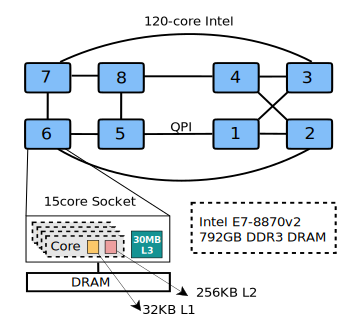
\includegraphics[width=0.3\textwidth]{fig/xeon}
  \end{center}
  \caption{Test-bed Intel Xeon architecture.}
  \label{fig:basic}
\end{figure}


측정 환경은 아래와 같다.

\begin{table}[h!]
  \centering
  \small
  \begin{tabular}{l l l l l} \toprule
    JVM & Spark & OS & Distribution\\
    \midrule
    Openjdk 1.8.0\_91 & 1.3.1 & 1.2.1 & Linux 4.5-rc6 & Ubuntu 14.04\\ 
    \bottomrule
  \end{tabular}
  \caption{System information and configuration values.}
  \label{tab:memuse}
\end{table}

\begin{figure*}[tb!]
    \centering
    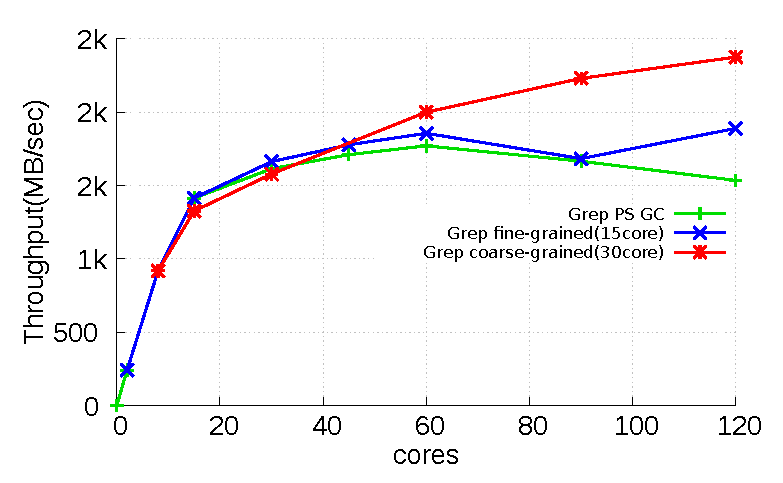
\includegraphics[width=4.8in]{graph/scalability.eps}
    \caption{Performance scalability using docker container.}
    \label{fig:docker}
\end{figure*}

\section{PARSEC 워크로드}
\begin{itemize}
    \item \textbf{Blackscholes.} 위 유의사항 3개항목을 제외한 논문작성폰트, 크기는 임의 사용가능합니다. 
    단, 논문집(Proceedings) 제작시 축소 인쇄하므로 글자크기를 9pt 이하는 사용하지 마시기 바랍니다.
    \item \textbf{Bodytrack.} 논문심사는 저자와 심사위원 상호 비공개로 진행됩니다. 
    따라서, 심사용(저자정보 삭제)과 출판용(저자정보 포함)으로 나눠 제출합니다. 
    심사용은 투고시, 출판용은 심사후 지정된 수정기간중에 각 업로드 하시면 됩니다. 
    \item \textbf{Bodytrack.} 논문심사는 저자와 심사위원 상호 비공개로 진행됩니다. 
    따라서, 심사용(저자정보 삭제)과 출판용(저자정보 포함)으로 나눠 제출합니다. 
    심사용은 투고시, 출판용은 심사후 지정된 수정기간중에 각 업로드 하시면 됩니다. 
    \item \textbf{Bodytrack.} 논문심사는 저자와 심사위원 상호 비공개로 진행됩니다. 
    따라서, 심사용(저자정보 삭제)과 출판용(저자정보 포함)으로 나눠 제출합니다. 
    심사용은 투고시, 출판용은 심사후 지정된 수정기간중에 각 업로드 하시면 됩니다. 
    \item \textbf{Bodytrack.} 논문심사는 저자와 심사위원 상호 비공개로 진행됩니다. 
    따라서, 심사용(저자정보 삭제)과 출판용(저자정보 포함)으로 나눠 제출합니다. 
    심사용은 투고시, 출판용은 심사후 지정된 수정기간중에 각 업로드 하시면 됩니다. 
\end{itemize}

\section{확장성 실험}

\section{PARSEC CPU 사용량 분석}



\section{결론 및 향후 연구}

\bibliographystyle{ieeetr}
\bibliography{ref}

\end{document}
